% Enable warnings about problematic code
\RequirePackage[l2tabu, orthodox]{nag}

\documentclass{resources/WeSTassignment}
\usepackage{tabularx}
\usepackage{booktabs}
\usepackage[utf8]{inputenc}
\usepackage{amsmath}
\usepackage{graphics}
\usepackage{graphicx}
\usepackage{changebar}
\usepackage{latexsym}
\usepackage{stmaryrd}
\usepackage{booktabs}
\usepackage{amsmath}
\usepackage{wasysym}
\usepackage[export]{adjustbox}
\usepackage[thinlines]{easytable}
\usepackage{framed}
\usepackage{color}
\usepackage{footnote}
\usepackage{listings}
\usepackage{framed}
\usepackage{tikz}
\usepackage[T1]{fontenc}
\usepackage{lmodern}
%\usepackage[table]{xcolor}

% The lecture title, e.g. "Web Information Retrieval".
\lecture{Introduction to Web Science}
% The names of the lecturer and the instructor(s)
\author{%
  PD Dr. Matthias~Thimm\\{\normalsize\mailto{thimm@uni-koblenz.de}} \and
  Ipek~Baris Schlicht\\{\normalsize\mailto{ibaris@uni-koblenz.de}} \and
  Kenneth Skiba\\{\normalsize\mailto{kennethskiba@uni-koblenz.de}}
}
% Assignment number.
\assignmentnumber{1}
% Institute of lecture.
\institute{%
  Institute of Web Science and Technologies\\%
  Department of Computer Science\\%
  University of Koblenz-Landau%
}
% Date until students should submit their solutions.
\datesubmission{17.11.2020, CEST 23:59}
% Date on which the assignments will be discussed in the tutorial.

% Specify bib file location.
\addbibresource{bibliography.bib}

\begin{document}

\maketitle

For the programming tasks, please do not add your code on the PDF. You need to submit only the .ipynb or .py files.

In case a team member has not contributed to the assignment, please do not include the name in the PDF. \\ 
\section{Introduction to Python Programming\hfill{20 points}}
\subsection{\hfill{10 points}}
In this task, you will write a simple python script that does the following:
\begin{enumerate}
    \item Generate a random number sequence of \textbf{100} values that are \textbf{between 0 to 1000}. Make sure that each of element in the sequence is type of \texttt{float} and use \textbf{42} as random seed. 
    \item Print each of the element in the sequence.
    \item The elements in the sequence denote the degrees. Perform sine and cosine operation on them and store the values in two different arrays named SIN and COS respectively.
    \item Plot the values of SIN and COS in two different colors and shapes. The plot must have labeled axes and legend that contain plausible information of the task. 
\end{enumerate}
Only \texttt{numpy}, \texttt{random} and \texttt{matplotlib} are allowed for this task. 

\subsection{\hfill{10 points}}
Write another simple python script that does the following:
\begin{enumerate}
    \item Read sample text (\texttt{sample.txt}) and store in \texttt{TEXT} variable.
    \item Count the frequency of each word in \texttt{TEXT} by filtering out any punctuation (e.g \texttt{.}, \texttt{!}) and number. If a word has uppercase letters, change them to lowercase.
    \item Plot the frequency distribution of words that occurs more than once, in an descending order. The plot must have labeled axes and legend that contain plausible information of the task. Apply the necessary settings for readable axes' information. 
\end{enumerate}
Only \texttt{string} and \texttt{matplotlib} are allowed for this task. 

For the programming tasks, you can use Google Colab. However, if you use your computer, make sure that the version of Python is 3.6 or 3.7.

\section{Ethernet Frame \hfill{20 points}}
An Ethernet Frame is of the given structure:
\begin{table}[h]
    \centering
    \scriptsize
    \begin{tabular}{|c|c|c|c|c|c|}
    \hline
         Preamble & Destination MAC address & Source MAC address & Type/Length & User Data & Frame Check Sequence  \\ \hline
         8 & 6 & 6 & 2 & 46-1500 & 4 \\ \hline
    \end{tabular}
    \caption{Ethernet Frame Structure with associated sizes in Bytes}
    \label{tab:ethernet_frame_structure}
\end{table}

Given below are two Ethernet frames.

    \texttt{aa aa aa aa aa aa aa ff} \hspace{2cm} \texttt{10 52 99 a5 42 d7 02 55} \\
    \texttt{74 31 59 a8 86 dd aa 31} \hspace{2cm} \texttt{89 45 63 81 23 05 03 88} \\
    \texttt{e2 41 31 83 b2 83 41 09} \hspace{2cm} \texttt{00 00 00 00 00 31 c0 a8} \\
    \texttt{02 67 00 00 18 ca 70 46} \\
    

    \texttt{aa aa aa aa aa aa aa ff} \hspace{2cm} \texttt{41 21 65 66 aa 01 41 92} \\
    \texttt{12 43 00 de 08 06 00 31} \hspace{2cm} \texttt{00 09 03 13 53 71 58 12} \\
    \texttt{97 53 13 12 54 13 90 31} \hspace{2cm} \texttt{00 00 00 00 00 31 c0 a8} \\ 
    \texttt{02 67 00 00 63 c5 63 3c} \\
    
    Find for both Ethernet frames:
    \begin{enumerate}
        \item Destination MAC Address
        \item Source MAC Address
        \item What protocol is inside the data payload?
    \end{enumerate}
    

\section{Research tasks \hfill {20 points}}
In this task you should do additional research extending the lecture. Please keep the citation rules in mind.
\subsection{Collision}
A computer tries to send data over an Ethernet network. However, after sending three packages the computer detects a collision.
What happens next? 

Describe in your own words how the Ethernet Collision Detection Algorithm handles a detected collision and highlight how the algorithm stops.

\subsection{IPv6}
In a few sentences please research the differences between IPv4 and IPv6 and explain the advantages of IPv6.

\section{Routing Table \hfill {20 points}}
\subsection{Solution:}
Based on the schematic representation from Figure \ref{fig:schematic_routing1} the routing table is as shown in table \ref{tab:routing_table1}
\begin{figure}[h]
    \centering
    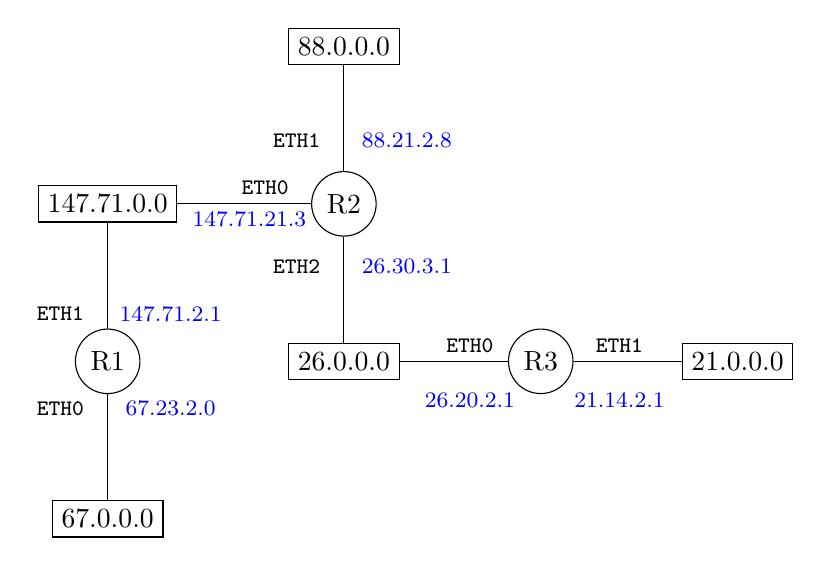
\begin{tikzpicture}
\node[draw, rectangle](C1) at (0,0) {67.0.0.0};
\node[draw, rectangle](C2) at (0,4) {147.71.0.0};
\node[draw, rectangle](C3) at (3,6) {88.0.0.0};
\node[draw, rectangle](C4) at (3,2) {26.0.0.0};
\node[draw, rectangle](C5) at (8,2) {21.0.0.0};

\node[draw, circle](R1) at (0,2) {R1};
\node[draw, circle](R2) at (3,4) {R2};
\node[draw, circle](R3) at (5.5,2) {R3};

\draw[-](C1) to (R1);
\node (R1_eth0) at (-0.6,1.4) {\texttt{\footnotesize{ETH0}}};
\node (R1_mac0) at (0.8,1.4) {\textcolor{blue}{\footnotesize{67.23.2.0}}};
\draw[-](R1) to (C2);
\node (R1_eth1) at (-0.6,2.6) {\texttt{\footnotesize{ETH1}}};
\node (R1_ma1) at (0.8,2.6) {\textcolor{blue}{\footnotesize{147.71.2.1}}};
\draw[-](C2) to (R2);
\node (R2_eth0) at (2,4.2) {\texttt{\footnotesize{ETH0}}};
\node (R2_mac0) at (1.8,3.8) {\textcolor{blue}{\footnotesize{147.71.21.3}}};
\draw[-](R2) to (C3);
\node (R2_eth1) at (2.4,4.8) {\texttt{\footnotesize{ETH1}}};
\node (R2_ma1) at (3.8,4.8) {\textcolor{blue}{\footnotesize{88.21.2.8}}};
\draw[-](R2) to (C4);
\node (R2_eth2) at (2.4,3.2) {\texttt{\footnotesize{ETH2}}};
\node (R2_ma2) at (3.8,3.2) {\textcolor{blue}{\footnotesize{26.30.3.1}}};
\draw[-](C4) to (R3);
\node (R3_eth0) at (4.6,2.2) {\texttt{\footnotesize{ETH0}}};
\node (R3_mac0) at (4.6,1.5) {\textcolor{blue}{\footnotesize{26.20.2.1}}};
\draw[-](R3) to (C5);
\node (R3_eth1) at (6.5,2.2) {\texttt{\footnotesize{ETH1}}};
\node (R3_mac1) at (6.5,1.5) {\textcolor{blue}{\footnotesize{21.14.2.1}}};
\end{tikzpicture}
    \caption{Routing schematic representation}
    \label{fig:schematic_routing1}
\end{figure}

\begin{table}[h]
\centering
\caption{Routing Table for \ref{fig:schematic_routing1}}
\label{tab:routing_table1}
\scalebox{0.8}{
\begin{tabular}{|l|l|l|l|l|l|l|l|l|}
\hline
\multicolumn{3}{|c|}{Router 1}        & \multicolumn{3}{c|}{Router 2}         & \multicolumn{3}{c|}{Router 3}        \\ \hline
Destination & Next Hop    & Interface & Destination & Next Hop    & Interface & Destination & Next Hop   & Interface \\ \hline
67.0.0.0    & 67.23.2.0   & eth0      & 147.71.0.0  & 147.71.21.3  & eth0      & 26.0.0.0  & 26.20.2.1 & eth0      \\ \hline
147.71.0.0    & 147.71.2.1   & eth1      & 88.0.0.0  & 88.21.2.8 & eth1      & 21.0.0.0    & 21.14.2.1  & eth1      \\ \hline
88.0.0.0  & 147.71.21.3 & eth1      & 26.0.0.0    & 26.30.3.1    & eth2      & 88.0.0.0    & 26.30.3.1 & eth0      \\ \hline
26.0.0.0    & 147.71.21.3 & eth1      & 67.0.0.0    & 141.71.2.1 & eth0      & 147.71.0.0  & 26.30.3.1  & eth0      \\ \hline
21.0.0.0 & 147.71.21.3   & eth1      & 21.0.0.0    & 26.20.2.1 & eth2      & 67.0.0.0    & 26.30.3.1  & eth0      \\ \hline
\end{tabular}
}
\end{table}

\subsection{Solution:}
The Routing schematic representation for table \ref{tab:routing_table2} is shown in figure \ref{fig:schematic_routing2}.\\
The steps in path traversal if a packet which is generated from 67.0.0.0 network and heading for 26.0.0.0 network are:
\begin{enumerate}
	\item When a packet is generated at \textbf{67.0.0.0} for destination \textbf{26.0.0.0}, the host will look up the routing table for the next hop which is at IP \textbf{67.68.3.1} through interface \textbf{eth0} in order to reach router 1 (represented by R1). 
	\item The router looks up the destination IP of the packet and confirm it's actual destination and lookup in the routing table for the next hop to reach that network which is \textbf{141.71.20.1} though interface \textbf{eth2} and reaches \textbf{147.71.0.0}. 
	\item Upon receiving this packet the network will repeat the process of looking up in the routing table and redirect to router 2 (represented by R2) by taking the next hop at \textbf{141.71.26.3} through interface \textbf{eth1}. 
	\item Since router 2 is directly connected to network \textbf{26.0.0.0} the last hop is taken at \textbf{26.3.2.1} through interface  \textbf{eth2}.
\end{enumerate}

The Routing schematic representation to send a packet which is generated from 67.0.0.0 network and heading for 26.0.0.0 network is shown in figure \ref{fig:schematic_routing3}.\\
\begin{table}[h]
\centering
\caption{Routing Table}
\label{tab:routing_table2}
\scalebox{0.8}{
\begin{tabular}{|l|l|l|l|l|l|l|l|l|}
\hline
\multicolumn{3}{|c|}{Router 1}        & \multicolumn{3}{c|}{Router 2}         & \multicolumn{3}{c|}{Router 3}        \\ \hline
Destination & Next Hop    & Interface & Destination & Next Hop    & Interface & Destination & Next Hop   & Interface \\ \hline
67.0.0.0    & 67.68.3.1   & eth0      & 205.30.7.0  & 205.30.7.1  & eth0      & 205.30.7.0  & 205.30.7.2 & eth0      \\ \hline
88.0.0.0    & 88.4.32.6   & eth1      & 141.71.0.0  & 141.71.26.3 & eth1      & 88.0.0.0    & 88.6.32.1  & eth1      \\ \hline
141.71.0.0  & 141.71.20.1 & eth2      & 26.0.0.0    & 26.3.2.1    & eth2      & 26.0.0.0    & 205.30.7.1 & eth0      \\ \hline
26.0.0.0    & 141.71.26.3 & eth2      & 67.0.0.0    & 141.71.20.1 & eth1      & 141.71.0.0  & 205.30.7.1  & eth0      \\ \hline
205.30.7.0  & 88.6.32.1   & eth1      & 88.0.0.0    & 141.71.20.1 & eth1      & 67.0.0.0    & 88.4.32.6  & eth1      \\ \hline
\end{tabular}
}
\end{table}

\begin{figure}[h]
    \centering
    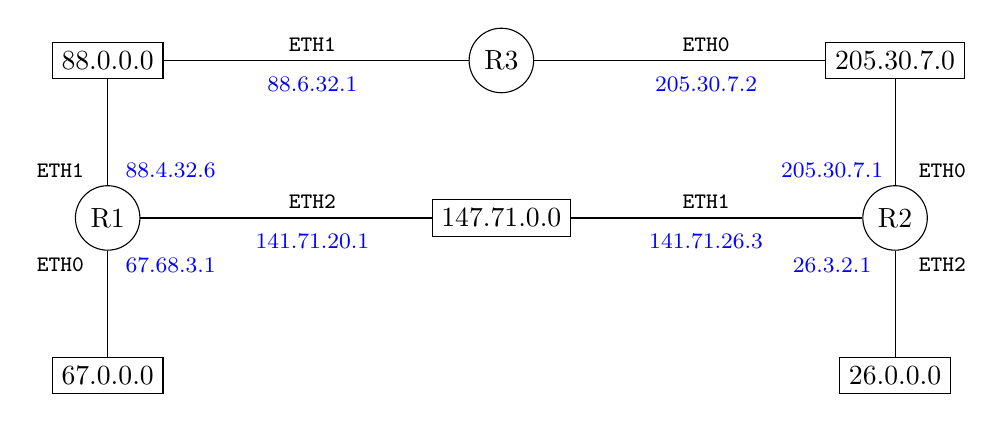
\begin{tikzpicture}
\node[draw, rectangle](C1) at (0,0) {67.0.0.0};
\node[draw, rectangle](C2) at (5,2) {147.71.0.0};
\node[draw, rectangle](C3) at (0,4) {88.0.0.0};
\node[draw, rectangle](C4) at (10,0) {26.0.0.0};
\node[draw, rectangle](C5) at (10,4) {205.30.7.0};

\node[draw, circle](R1) at (0,2) {R1};
\node[draw, circle](R2) at (10,2) {R2};
\node[draw, circle](R3) at (5,4) {R3};

\draw[-](C1) to (R1);
\node (R1_eth0) at (-0.6,1.4) {\texttt{\footnotesize{ETH0}}};
\node (R1_mac0) at (0.8,1.4) {\textcolor{blue}{\footnotesize{67.68.3.1}}};
\draw[-](R1) to (C3);
\node (R1_eth1) at (-0.6,2.6) {\texttt{\footnotesize{ETH1}}};
\node (R1_ma1) at (0.8,2.6) {\textcolor{blue}{\footnotesize{88.4.32.6}}};
\draw[-](R1) to (C2);
\node (R1_eth2) at (2.6,2.2) {\texttt{\footnotesize{ETH2}}};
\node (R1_ma2) at (2.6,1.7) {\textcolor{blue}{\footnotesize{141.71.20.1}}};

\draw[-](C5) to (R2);
\node (R2_eth0) at (10.6,2.6) {\texttt{\footnotesize{ETH0}}};
\node (R2_mac0) at (9.2,2.6) {\textcolor{blue}{\footnotesize{205.30.7.1}}};
\draw[-](R2) to (C2);
\node (R2_eth1) at (7.6,2.2) {\texttt{\footnotesize{ETH1}}};
\node (R2_mac1) at (7.6,1.7) {\textcolor{blue}{\footnotesize{141.71.26.3}}};
\draw[-](R2) to (C4);
\node (R2_eth2) at (10.6,1.4) {\texttt{\footnotesize{ETH2}}};
\node (R2_ma2) at (9.2,1.4) {\textcolor{blue}{\footnotesize{26.3.2.1}}};

\draw[-](R3) to (C5);
\node (R3_eth0) at (7.6,4.2) {\texttt{\footnotesize{ETH0}}};
\node (R3_ma0) at (7.6,3.7) {\textcolor{blue}{\footnotesize{205.30.7.2}}};
\draw[-](C3) to (R3);
\node (R3_eth1) at (2.6,4.2) {\texttt{\footnotesize{ETH1}}};
\node (R3_mac1) at (2.6,3.7) {\textcolor{blue}{\footnotesize{88.6.32.1}}};
\end{tikzpicture}
    \caption{Routing schematic representation}
    \label{fig:schematic_routing2}
\end{figure}
\begin{figure}[h]
	\centering
	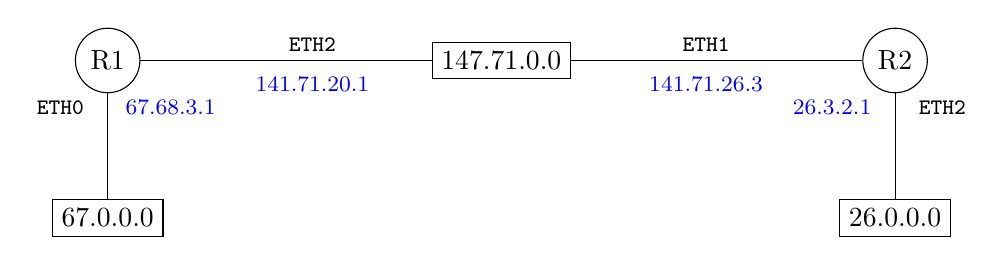
\begin{tikzpicture}
\node[draw, rectangle](C1) at (0,0) {67.0.0.0};
\node[draw, rectangle](C2) at (5,2) {147.71.0.0};
\node[draw, rectangle](C4) at (10,0) {26.0.0.0};

\node[draw, circle](R1) at (0,2) {R1};
\node[draw, circle](R2) at (10,2) {R2};

\draw[-](C1) to (R1);
\node (R1_eth0) at (-0.6,1.4) {\texttt{\footnotesize{ETH0}}};
\node (R1_mac0) at (0.8,1.4) {\textcolor{blue}{\footnotesize{67.68.3.1}}};

\draw[-](R1) to (C2);
\node (R1_eth2) at (2.6,2.2) {\texttt{\footnotesize{ETH2}}};
\node (R1_ma2) at (2.6,1.7) {\textcolor{blue}{\footnotesize{141.71.20.1}}};

\draw[-](R2) to (C2);
\node (R2_eth1) at (7.6,2.2) {\texttt{\footnotesize{ETH1}}};
\node (R2_mac1) at (7.6,1.7) {\textcolor{blue}{\footnotesize{141.71.26.3}}};
\draw[-](R2) to (C4);
\node (R2_eth2) at (10.6,1.4) {\texttt{\footnotesize{ETH2}}};
\node (R2_ma2) at (9.2,1.4) {\textcolor{blue}{\footnotesize{26.3.2.1}}};

\end{tikzpicture}
    \caption{Routing schematic representation of path if a packet is generated from 67.0.0.0 network and heading for 26.0.0.0 network.}
    \label{fig:schematic_routing3}
\end{figure}


 \section*{Important Notes}


  \subsection*{Submission}

  \begin{itemize}
    \item Solutions have to be submitted to the SVN repository.
      Use the directory name \texttt{groupname/assignment\@assignmentnumber{}/}
      in your group's repository.
%     \item The answer sheet must have the screenshots and the code where ever asked. 		Additional python \texttt{.py} file needs to be also added in the repository. 
    \item The name of the group and the names of all participating students must
      be listed on each submission.
      
%     \item With the submission of your solution you confirm that you created the
%       solution independently as a group, especially without using other
%       intellectual contributions.
%       In other words, you submission should not be
%       \href{https://en.wikipedia.org/wiki/Plagiarism}{plagiarism}!
%       Should the case occur that the submissions of multiple groups are
%       identical, none of these groups will receive credit.
    \item Solution format: all solutions as \emph{one} PDF document.
      Programming code has to be submitted as Python code to the SVN repository.
      Upload \emph{all} \texttt{.py} files of your program!
      Use \texttt{UTF-8} as the file encoding.
      \emph{Other encodings will not be taken into account!}
    \item Check that your code compiles without errors.
    \item Make sure your code is formatted to be easy to read.
      \begin{itemize}
        \item Make sure you code  has consistent
          \href{https://en.wikipedia.org/wiki/Indent_style}{indentation}.
        \item Make sure you comment and document your code
          adequately in English.
        \item Choose consistent and intuitive names for your identifiers.
      \end{itemize}
    \item Do \emph{not} use any accents, spaces or special characters in your
      filenames.
  \end{itemize}

%   \clearpage
  \subsection*{Acknowledgment}
	
    This pdfLaTeX template was adapted by Jun Sun based on the LuaLaTeX version by Lukas Schmelzeisen. 

\subsection*{\LaTeX}
Use \texttt{pdflatex or LuaLatex combiler for  assignment\_X.tex}  to build your PDF.


\end{document}